\section{Используемые технологии}
\label{sec:techs:intro}

Выбор технологий является важным предварительным этапом разработки сложных информационных систем.
Платформа и язык программирования, на котором будет реализована система, заслуживает большого внимания, так как исследования показали, что выбор языка программирования влияет на производительность труда программистов и качество создаваемого ими кода~\cite[c.~59]{mcconnell_2005}.

Ниже перечислены некоторые факторы, повлиявшие на выбор технологий:
\begin{itemize}
\item Разрабатываемое ПО должно работать на операционных системах Linux и Windows.
\item Программное средство должно быть выполнено в виде клиент-серверного приложения.
\item Дальнейшей поддержкой проекта, возможно, будут заниматься разработчики, не принимавшие участие в выпуске первой версии.
\item Имеющийся разработчик имеет опыт работы с объектно"=ориентированными и с функциональными языками программирования.
\end{itemize}

Основываясь на приведенных факторах, целесообразно выбрать в качестве платформы разработки язык Python. Приняв во внимание необходимость обеспечения доступности дальнейшей поддержки ПО, возможно, другой командой программистов, целесообразно не использовать малоизвестные и сложные языки программирования.

Для реализации поставленной задачи существует необходимость в написании серверного приложения. Эту задачу можно облегчить путём использования набора прикладных библотек (фреймворка) Flask, предназначенного для быстрого прототипирования и реализации веб-приложений различной степени сложности.

Далее проводится характеристика используемых технологий и языков программирования более подробно.



\subsection{Язык программирования Python}
\label{sub:techs:python}
Python — высокоуровневый язык программирования общего назначения, ориентированный на повышение производительности разработчика и читаемости кода. Синтаксис ядра Python минималистичен. В то же время стандартная библиотека включает большой объём полезных функций.

Python поддерживает несколько парадигм программирования, в том числе структурное, объектно-ориентированное, функциональное, императивное и аспектно-ориентированное. Основные архитектурные черты — динамическая типизация, автоматическое управление памятью, полная интроспекция, механизм обработки исключений, поддержка многопоточных вычислений и удобные высокоуровневые структуры данных. Код в Python организовывается в функции и классы, которые могут объединяться в модули (они в свою очередь могут быть объединены в пакеты).

Эталонной реализацией Python является интерпретатор CPython, поддерживающий большинство активно используемых платформ. Он распространяется под свободной лицензией Python Software Foundation License, позволяющей использовать его без ограничений в любых приложениях, включая проприетарные. Есть реализации интерпретаторов для JVM (с возможностью компиляции), MSIL (с возможностью компиляции), LLVM и других. Проект PyPy предлагает реализацию Python на самом Python, что уменьшает затраты на изменения языка и постановку экспериментов над новыми возможностями.

Python — активно развивающийся язык программирования, новые версии (с добавлением/изменением языковых свойств) выходят примерно раз в два с половиной года. Вследствие этого и некоторых других причин на Python отсутствуют стандарт ANSI, ISO или другие официальные стандарты, их роль выполняет CPython.

Отличительные особенности языка Python:
\begin{itemize}
  \item Простой. Python – простой и минималистичный язык. Чтение хорошей программы на Python очень напоминает чтение английского текста. Такая псевдо-кодовая природа Python является одной из его самых сильных сторон. Она позволяет сосредоточиться на решении задачи, а не на самом языке.
  \item Свободный и открытый. Python – это пример свободного и открытого программного обеспечения – FLOSS (Free/Libré and Open Source Software). Пользователь имеет право свободно распространять копии этого программного обеспечения, читать его исходные тексты, вносить изменения, а также использовать его части в своих программах. В основе свободного ПО лежит идея сообщества, которое делится своими знаниями. Это одна из причин, по которым Python так хорош: он был создан и постоянно улучшается сообществом, которое хочет сделать его лучше.
  \item Язык высокого уровня. При написании программы на Python разработчику не нужно отвлекаться на такие низкоуровневые детали, как управление памятью и т.п.
  \item Портируемый. Благодаря своей открытой природе, Python был портирован на множество платформ. Программы на Python могут запускаться на любой из этих платформ без каких-либо изменений (если программа не использует системно-зависимые функции). Python можно использовать в GNU/Linux, Windows, FreeBSD, Macintosh, Solaris, OS/2, Amiga, AROS, AS/400, BeOS, OS/390, z/OS, Palm OS, QNX, VMS, Psion, Acorn RISC OS, VxWorks, PlayStation, Sharp Zaurus, Windows CE и множестве других платформ.
  \item Интерпретируемый. Python не требует компиляции в бинарный код. Программа выполняется из исходного текста. Python сам преобразует этот исходный текст в некоторую промежуточную форму, называемую байткодом, а затем переводит его на машинный язык и запускает. Всё это заметно облегчает использование Python, поскольку нет необходимости заботиться о компиляции программы, подключении и загрузке нужных библиотек и т.д. Вместе с тем, это делает программы на Python намного более переносимыми.
  \item Объектно-ориентированный. Python поддерживает как процедурно-ориентированное, так и объектно-ориентированное программирование. Python предоставляет простые, но мощные средства для ООП, особенно в сравнении с такими большими языками программирования, как C++ или Java.
  \item Расширяемый. Если необходимо добиться очень высокой производительности некоторой части программы или использовать некоторые другие возможности более низкоуровневых языков, можно разработать эту часть программы на C или C++, а затем вызывать её из программы на Python.
  \item Встраиваемый. Python можно встраивать в программы на C/C++, чтобы предоставлять возможности написания сценариев их пользователям.
  \item Обширные библиотеки. Стандартная библиотека Python просто огромна. Она может помочь в решении самыхразнообразных задач, связанных с использованием регулярных выражений, генериро-ванием документации, проверкой блоков кода, распараллеливанием процессов, база-ми данных, веб-браузерами, CGI, FTP, электронной почтой, XML, XML-RPC, HTML, WAV файлами, криптографией, GUI и другими системно-зависимыми вещами. Всё это доступно абсолютно везде, где установлен Python. В этом заключается философия Python <<Всё включено>>.Кроме стандартной библиотеки, существует множество других высококачественных биб-лиотек, доступных в каталоге пакетов.
\end{itemize}

\subsubsection{Объектно-ориентированное программирование}
Дизайн языка Python построен вокруг объектно-ориентированной модели программирования. Реализация ООП в Python является элегантной, мощной и хорошо продуманной, но вместе с тем достаточно специфической по сравнению с другими объектно-ориентированными языками. Особенности~\cite{wiki_python, byte_of_python}:
\begin{itemize}
\item Классы являются одновременно объектами со всеми ниже приведёнными возможностями.
\item Наследование, в том числе множественное.
\item Полиморфизм (все функции виртуальные).
\item Инкапсуляция (два уровня — общедоступные и скрытые методы и поля). Особенность — скрытые члены доступны для использования и помечены как скрытые лишь особыми именами.
\item Специальные методы, управляющие жизненным циклом объекта: конструкторы, деструкторы, распределители памяти.
\item Перегрузка операторов (всех, кроме is, '.', '=' и символьных логических).
\item Свойства (имитация поля с помощью функций).
\item Управление доступом к полям (эмуляция полей и методов, частичный доступ, и т. п.).
\item Методы для управления наиболее распространёнными операциями (истинностное значение, len(), глубокое копирование, сериализация, итерация по объекту, …)
\item Метапрограммирование (управление созданием классов, триггеры на создание классов, и др.)
\item Классовые и статические методы, классовые поля.
\end{itemize}

\subsubsection{Функциональное программирование}
Python поддерживает парадигму функционального программирования, в частности:
\begin{itemize}
\item Функция является объектом;
\item Функции высших порядков;
\item Рекурсия;
\item Развитая обработка списков (списочные выражения, операции над последовательностями, итераторы);
\item Аналог замыканий;
\item Частичное применение функции;
\end{itemize}

\subsubsection{Интроспекция}
Python поддерживает полную интроспекцию времени исполнения. Это означает, что для любого объекта можно получить всю информацию о его внутренней структуре.
Применение интроспекции является важной частью того, что называют pythonic style, и широко применяется в библиотеках и фреймворках Python, таких как PyRO, PLY, Cherry, Django и др., значительно экономя время использующего их программиста.

\subsubsection{Итераторы и генераторы}
В программах на Python широко используются итераторы. Цикл for может работать как с последовательностью, так и с итератором. Все коллекции, как правило, предоставляют итератор. Объекты определённого пользователем класса тоже могут быть итераторами. Подробнее об итераторах можно узнать в разделе о функциональном программировании. Модуль itertools стандартной библиотеки содержит много полезных функций для работы с итераторами.

Другой интересной возможностей языка являются генераторы — функции, сохраняющие внутреннее состояние: значения локальных переменных и текущую инструкцию. Генераторы могут использоваться как итераторы для структур данных и для ленивых вычислений.
При вызове генератора функция немедленно возвращает объект-итератор, который хранит текущую точку исполнения и состояние локальных переменных функции. При запросе следующего значения (посредством метода next(), неявно вызываемого в цикле for) генератор продолжает исполнение функции от предыдущей точки останова до следующего оператора yield или return.


\subsection{Sandia National Laboratories PUF Analysis Tool (SPAT)}
\label{sec:techs:spat}
Sandia National Laboratories PUF Analysis Tool - программное средство с открытым исходным кодом, созданное Sandia Corporation для симуляции физически неклонируемых функций, наглядной демонстрации и оценки их статистических свойств. Этот инструмент был создан главным образом для использования в образовательных целях.

Функции данной программы не ограничиваются только лишь симуляцией, она с равным успехом может анализировать статистические свойства реальных физических PUF.
Программа представляет собой набор следующих модулей:
\begin{itemize}
  \item модуль взаимодействия с физическими устройствами;
  \item модуль симуляции PUF (может быть расширен пользователем);
  \item модуль анализа свойств PUF независимо от реализации (физическая или симуляция).
  \item графический интерфейс
\end{itemize}
SPAT может быть использована для визуализации:
\begin{itemize}
  \item влияния шума на выходной сигнал PUF;
  \item метрик среднего значени шума в микросхеме;
  \item динамики расстояния Хэмминга выходного сигнала в зависимости от динамики входного.
  \item свойств случайности для данного чипа, таких как энтропия.
\end{itemize}
\begin{figure}[ht]
    \centering
    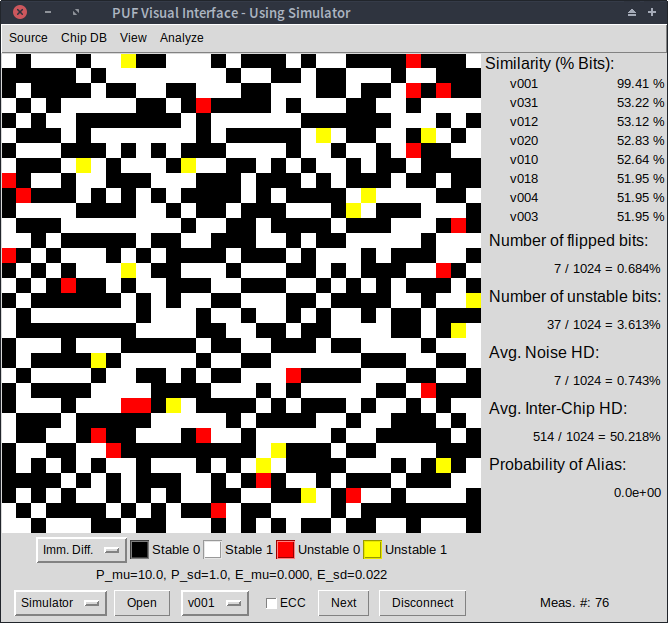
\includegraphics[width=0.7\textwidth]{spat.png}
    \caption{Окно программы SPAT с результатами статистического анализа виртуальной RO-PUF}
    \label{fig:techs:spat}
\end{figure}
